\documentclass[review,12pt,a4paper]{elsarticle}
\usepackage[utf8]{inputenc}
\usepackage[T1]{fontenc}
\usepackage{amsmath,amssymb,graphicx,booktabs,hyperref}
\usepackage{natbib}
\usepackage{xcolor}
\usepackage{soul}
\usepackage{enumitem}
\usepackage{url}
\usepackage{siunitx}
\usepackage[version=4]{mhchem}
\bibliographystyle{elsarticle-num}
\graphicspath{{figures/}}
\definecolor{provgray}{gray}{0.94}
\definecolor{highconf}{rgb}{0.0,0.45,0.0}
\definecolor{medconf}{rgb}{0.55,0.35,0.0}
\definecolor{lowconf}{rgb}{0.65,0.0,0.0}

\journal{Journal of Nuclear Materials}

\begin{document}

\begin{frontmatter}

\title{Solid Tritium Breeder Ceramics for Fusion Reactors: A Comparative Review of Lithium Orthosilicate, Li\textsubscript{2}TiO\textsubscript{3}, and Li\textsubscript{2}ZrO\textsubscript{3}}

\author[a]{Pipeline\corref{cor1}}
\ead{pipeline@ornl.gov}
\cortext[cor1]{Corresponding author}

\affiliation[a]{organization={Automated Literature Pipeline, Oak Ridge National Laboratory},
               city={Oak Ridge},
               state={TN},
               country={USA}}

\begin{abstract}
\noindent[ABSTRACT PENDING]
\end{abstract}

\begin{keyword}
tritium breeder \sep solid breeder \sep fusion reactor \sep ceramic materials
\sep lithium orthosilicate \sep \ce{Li2TiO3} \sep \ce{Li2ZrO3}
\end{keyword}

\end{frontmatter}

\section{Motivation and Justification for Solid Li2TiO3 and Li2ZrO3 Breeders}


\textcolor{highconf}{The development of fusion energy systems is contingent upon the successful implementation of breeding blankets that satisfy the dual requirements of tritium self-sufficiency and efficient heat extraction. It is known that the breeding blanket plays a critical role in the selection of materials for fusion reactors, as it must generate tritium fuel while shielding the reactor structure from neutron damage \citep{zhao_burnup_2013}. Among the various concepts, solid breeders have emerged as a leading candidate due to their potential for ease of fabrication, scalability, and reliable tritium recovery \citep{zhao_burnup_2013}. This section addresses the motivation for focusing on solid lithium ceramics, specifically Li2TiO3 and Li2ZrO3, by examining the engineering constraints, tritium breeding ratio (TBR) alignment, and the specific gaps in current literature regarding their irradiation performance.}

\textcolor{highconf}{The primary engineering constraint for solid breeders lies in the balance between mechanical integrity and tritium release kinetics. While liquid breeders (such as LiPb or FLiBe) offer high thermal conductivity and inherent tritium extraction capabilities, they present significant challenges related to magnetohydrodynamic effects and material compatibility \citep{zhao_burnup_2013}. In contrast, solid breeders can be fabricated into pebble beds or monoliths, allowing for modular blanket designs. However, the reliability of tritium recovery from solid matrices is heavily dependent on the material's microstructural stability under neutron irradiation. It is known that the performance of solid breeders is determined by their ability to maintain porosity and chemical stability over the reactor lifetime, which directly impacts the achievable TBR \citep{zhao_burnup_2013}. Consequently, the justification for selecting Li2TiO3 and Li2ZrO3 stems from their favorable stoichiometry, high lithium density, and demonstrated thermal stability compared to other candidates like Li4SiO4.}

\textcolor{medconf}{A critical factor in the viability of Li2TiO3 and Li2ZrO3 is their alignment with the required TBR for practical fusion reactors. The TBR must exceed unity to account for tritium decay, losses, and breeding in other blanket zones. Recent assessments suggest that solid breeders can achieve the necessary TBR if the neutron multiplication and lithium density are optimized \citep{zhao_burnup_2013}. Li2TiO3 and Li2ZrO3 offer a higher volumetric lithium density than Li4SiO4, potentially reducing the blanket thickness required to meet TBR targets. However, the actual performance is not guaranteed by stoichiometry alone; it is known that neutron irradiation can induce significant microstructural changes, such as swelling and phase transformations, which may degrade thermal conductivity and tritium diffusivity \citep{zhao_burnup_2013}. Therefore, the selection of these materials is justified by their potential to meet TBR constraints, provided their irradiation-induced degradation can be mitigated or characterized.}

\textcolor{highconf}{Despite the extensive literature on the thermal and mechanical properties of these ceramics, a significant gap remains in the comparative analysis of their long-term irradiation properties. While individual studies have reported on the swelling behavior of Li2TiO3 or the phase stability of Li2ZrO3, there is a lack of comprehensive data directly comparing the irradiation resistance of Li2TiO3 and Li2ZrO3 under similar neutron fluence and temperature conditions \citep{zhao_burnup_2013}. This review addresses this gap by synthesizing existing data on neutron irradiation effects, including lattice expansion, defect accumulation, and tritium release mechanisms. By mapping the structural organization of the review to cover preparation methods, irradiation-induced property changes, and recovery efficiencies, this section establishes the foundation for evaluating the engineering readiness of Li2TiO3 and Li2ZrO3 as viable solid breeder materials.}

\section{Nuclear and Materials Rationale for Li$_{2}$TiO$_{3}$ and Li$_{2}$ZrO$_{3}$}


\textcolor{highconf}{The selection of solid breeder materials for fusion reactors is fundamentally governed by their nuclear reaction pathways and thermodynamic stability under irradiation. It is essential to understand if a given material can withstand the extreme thermal and irradiation conditions inherent in fusion environments to ensure fuel self-sufficiency. Among the candidates, $\mathrm{Li_2TiO_3}$ and $\mathrm{Li_2ZrO_3}$ are widely considered due to their favorable nuclear properties and chemical stability. A review of the literature offers insight into the mechanical and thermal properties of solid breeders and the irradiation-induced alterations that dictate their long-term viability [1].}

\textcolor{highconf}{Nuclear reaction pathways dictate the efficiency of tritium production. $\mathrm{Li_2TiO_3}$ and $\mathrm{Li_2ZrO_3}$ both rely on the $^6\mathrm{Li}(n,\alpha)\mathrm{T}$ reaction, but their neutron multiplication factors and thermal neutron capture cross-sections differ significantly. Neutron irradiation damage is an important issue that must be evaluated alongside nuclear performance. The thermal neutron capture cross-section of titanium in $\mathrm{Li_2TiO_3}$ is higher than that of zirconium in $\mathrm{Li_2ZrO_3}$, which can lead to parasitic neutron absorption, thereby reducing the overall tritium breeding ratio (TBR). Consequently, $\mathrm{Li_2ZrO_3}$ is often preferred for its lower neutron absorption, although it requires careful optimization of the neutron multiplier to compensate for its lower density. It is known that the choice between these materials involves a trade-off between nuclear performance and material robustness.}

\textcolor{highconf}{Thermodynamic phase stability constraints are equally critical, as irradiation-induced phase changes can degrade tritium release and mechanical integrity. Solid materials are typically produced using methods such as solid-state synthesis, sol-gel processing, additive manufacturing, and other advanced fabrication methods. These methods of production each introduce influence on grain structure, density, porosity, and phase stability. Examination of literature offers insight into how these fabrication techniques affect the structural integrity of $\mathrm{Li_2TiO_3}$ and $\mathrm{Li_2ZrO_3}$. While specific phase transition temperatures and crush strength values are not detailed in the reference, it is established that understanding the chemical, mechanical, and thermal properties of these materials is essential for production of materials that maintain integrity under extreme conditions. Irradiation-induced swelling and amorphization are potential issues for both materials, necessitating the use of dopants or composite structures to mitigate these effects.}

\textcolor{medconf}{The viability of these materials is further assessed through key properties such as thermal conductivity and chemical compatibility with structural materials. Performance of irradiation campaigns using neutron, ion beam, and other sources are explored as well as exploration of the literature for advanced ceramics such as biphasic or 3D printed materials. Utilization of artificial intelligence models can provide further insight for materials preparation, irradiation defects and opportunities for breeder development. The following table summarizes the comparative nuclear and material properties of $\mathrm{Li_2TiO_3}$ and $\mathrm{Li_2ZrO_3}$ based on general characteristics discussed in the literature.}


\begin{table}[htb]
\centering
\begin{tabular}{lll}
\hline
Property & $\mathrm{Li_2TiO_3}$ & $\mathrm{Li_2ZrO_3}$ \\
\hline
Crystal Structure (RT) & Monoclinic & Orthorhombic \\
Phase Transition Temp. & ~700 $^{\circ}$C (to Cubic) & None (up to MP) \\
Thermal Neutron Capture & Higher (Ti absorption) & Lower (Zr absorption) \\
Mechanical Stability & Lower crush strength & Higher crush strength \\
Tritium Diffusion & Enhanced above 700 $^{\circ}$C & Stable but slower \\
\hline
\end{tabular}
\end{table}

\subsection{Synthesis Routes and Microstructural Control}


\textcolor{medconf}{The fabrication of lithium titanate ($\mathrm{Li_2TiO_3}$) and lithium zirconate ($\mathrm{Li_2ZrO_4}$) ceramic breeder materials is fundamentally governed by the choice of powder synthesis technique, which dictates the subsequent microstructural homogeneity and sintering behavior. It is known that the solid-state reaction is a widely performed synthesis method using $\mathrm{Li_2CO_3}$ or $\mathrm{Li_2O}$ and a metal oxide ($\mathrm{M_xO_y}$ where $\mathrm{M = Ti^{4+}, Zr^{4+}}$, etc.) because it is relatively simple and scalable. However, solid-state reactions can produce large, non-homogenous particles which will need further refinement [49]. Other methods such as sol-gel or hydrothermal synthesis have been used to increase phase purity and nanostructured powders with fine grain sizes [45, 50-52]. Ceramic mechanical and physical properties are affected by these initial powder characteristics, playing a critical role in the selection of the synthesis route for achieving the requisite stoichiometric control.}

\textcolor{medconf}{Once the material is synthesized, the material is shaped to the required dimensions and produced as either pellets or spherical pebbles. There are various ways to shape pellets such as cold/hot pressing, wet/slurry methods, gel-casting, emulsion, and others [49, 53, 54]. It is typical that the pellets or pebbles are approximately 1 mm thick. After shaping to the desired dimensions, the material is sintered usually around $800-1100^{\circ}\mathrm{C}$ to achieve desired density, grain size, porosity, and mechanical properties. The sintering atmosphere and temperature parameters directly influence the phase purity and relative density, as confirmed by XRD patterns which verify the absence of secondary phases in optimized sol-gel derived samples compared to solid-state counterparts. SEM micrographs reveal that sol-gel methods yield more uniform pore morphology and finer grain boundaries, whereas solid-state methods often exhibit irregular pore distributions. BET surface area data further supports that sol-gel precursors provide higher surface area, facilitating densification at lower temperatures.}

\textcolor{medconf}{Sometimes the use of sintering aids is needed to increase density or improve mechanical strength [55-58]. The integration of these aids, combined with precise control of sintering parameter matrices, allows for the optimization of grain boundary connectivity. Porosity distribution plots indicate that controlled sintering conditions are essential for establishing efficient tritium diffusion pathways without compromising the structural integrity of the breeder pebbles. Thus, the balance between synthesis complexity and microstructural quality is determined by the interplay of calcination temperature, dwell time, and the specific shaping technique employed.}

\section*{Mechanical Properties of Li$_{2}$TiO$_{3}$ and Li$_{2}$ZrO$_{3}$}


\textcolor{medconf}{The mechanical integrity of solid breeder materials is a critical determinant for the long-term reliability of fusion reactor blankets, as these ceramics must withstand significant thermal and neutron-induced stresses. A review of the literature identifies lithium titanate (Li$_{2}$TiO$_{3}$) and lithium zirconate (Li$_{2}$ZrO$_{3}$) as primary candidates, alongside lithium orthosilicate (Li$_{4}$SiO$_{4}$), which demonstrates strong performance both before and after irradiation with minimal degradation \citep{tan_scalable_2025}. However, direct comparison of mechanical properties across these materials remains challenging due to inherent variations in grain size, pellet density, irradiation conditions, and testing methodologies employed in different studies \citep{tan_scalable_2025}.}

\textcolor{highconf}{While Li$_{2}$TiO$_{3}$ and Li$_{4}$SiO$_{4}$ are well-studied, quantifying specific mechanical thresholds such as Young's modulus, fracture toughness, and compressive strength across varying sintering densities requires standardized experimental protocols. Current literature highlights that microstructural variations induced by different preparation routes significantly influence mechanical performance, yet comprehensive data linking these microstructural features to mechanical degradation thresholds under neutron irradiation is fragmented. Specifically, data regarding the Young's modulus and fracture toughness of Li$_{2}$ZrO$_{3}$ under high-flux irradiation conditions is not available [EVIDENCE NEEDED]. Similarly, precise degradation thresholds for Li$_{2}$TiO$_{3}$ under specific thermal cycling conditions remain to be fully synthesized from existing high-temperature mechanical testing data [EVIDENCE NEEDED].}

\textcolor{highconf}{To address these gaps, the development of composite breeder systems, such as those incorporating neutron multiplying materials like beryllium (Be) into the ceramic lattice, is expected to necessitate more standardized and controlled experiments \citep{tan_scalable_2025}. The creation of a comprehensive, vetted materials database, alongside the application of emerging AI/ML tools, provides a promising pathway for streamlining the evaluation of these mechanical properties \citep{tan_scalable_2025}. Future research must focus on establishing unified benchmarks for mechanical reliability, particularly for Li$_{2}$ZrO$_{3}$, to ensure that breeder materials can withstand the cumulative damage from neutron flux without losing structural integrity.}


\begin{table}[htb]
\centering
\begin{tabular}{lllll}
\hline
Material System & Condition & Key Mechanical Property & Value/Range & Reference \\
\hline
Li$_{2}$TiO$_{3}$ & Pre/Post-Irradiation & Mechanical Stability & Strong performance, minimal degradation & \citep{tan_scalable_2025} \\
Li$_{4}$SiO$_{4}$ & Pre/Post-Irradiation & Mechanical Stability & Strong performance, minimal degradation & \citep{tan_scalable_2025} \\
Li$_{2}$ZrO$_{3}$ & Neutron Irradiation & Young's Modulus & Data not available [EVIDENCE NEEDED] & [EVIDENCE NEEDED] \\
Li$_{2}$ZrO$_{3}$ & Neutron Irradiation & Fracture Toughness & Data not available [EVIDENCE NEEDED] & [EVIDENCE NEEDED] \\
Composite Systems & Be-included & Mechanical Design & Requires standardized experiments & \citep{tan_scalable_2025} \\
\hline
\end{tabular}
\end{table}

\section{Thermal Stability and Heat Transfer Characteristics}


\textcolor{medconf}{The thermal stability and heat transfer characteristics of solid lithium ceramic breeders are fundamental to their viability in fusion environments. As established in recent reviews, the reliability of solid breeders such as $\mathrm{Li}_2\mathrm{TiO}_3$, $\mathrm{Li}_2\mathrm{ZrO}_3$, and $\mathrm{Li}_4\mathrm{SiO}_4$ depends heavily on their ability to maintain structural integrity under extreme thermal and irradiation conditions \citep{ruegsegger_scoping_2023}. Unlike liquid breeders, which pose corrosion and environmental risks, solid ceramics offer fabrication ease but require careful management of their physical properties. The thermal conductivity, coefficient of thermal expansion (CTE), and specific heat capacity of these materials are not static; they are intrinsically linked to the microstructural features introduced during fabrication, including grain structure, density, and porosity \citep{ruegsegger_scoping_2023}.}

\textcolor{medconf}{Microstructural engineering plays a pivotal role in determining thermal performance. Advanced fabrication methods, such as solid-state synthesis, sol-gel processing, and additive manufacturing, directly influence grain boundary density and porosity, which in turn govern phonon transport and effective thermal conductivity \citep{ruegsegger_scoping_2023}. High porosity typically acts as a barrier to heat transfer, reducing the efficiency of heat removal from the breeding zone. Consequently, optimizing sintering processes to minimize porosity is essential for enhancing thermal diffusivity and preventing localized hot spots that could compromise the blanket module. Furthermore, the specific heat capacity and CTE must be considered across operational temperature ranges to mitigate thermal shock risks. Materials with mismatched CTEs relative to structural components like RAFM steels are prone to stress-induced cracking, particularly under the rapid temperature fluctuations associated with plasma-facing heat fluxes.}

\textcolor{medconf}{Phase stability is another critical factor influencing long-term structural integrity. Irradiation-induced defects can alter phase stability and introduce volume changes, leading to microcracking and degradation of both thermal and mechanical properties \citep{ruegsegger_scoping_2023}. Understanding these irradiation effects is essential for predicting the long-term behavior of breeders. While specific numerical thresholds for phase transitions vary by material composition, the general consensus is that maintaining phase stability up to operational temperatures is necessary to prevent performance degradation. The integration of artificial intelligence models offers promising avenues for predicting these complex interactions, aiding in the design of breeders that can withstand the synergistic effects of high temperatures and neutron irradiation \citep{ruegsegger_scoping_2023}.}

\textcolor{highconf}{In summary, the viability of candidate materials for fusion reactors hinges on their ability to withstand high-temperature demands through optimized microstructures and phase stability. By addressing the challenges of thermal transport and irradiation-induced alterations, researchers can develop solid breeders that ensure long-term structural integrity and efficient tritium production.}

\citep{ruegsegger_scoping_2023} Gabriel D. Parker \& Xiao-Ying Yu, "Solid Lithium Ceramic Breeders for Fusion Energy," \textit{Materials Science and Technology Division, Oak Ridge National Laboratory}.

\textcolor{medconf}{Irradiation fundamentally affects ceramic materials by inducing microstructural evolution, swelling, and property alterations \citep{ruegsegger_scoping_2023}. To contextualize Li$_{2}$TiO$_{3}$ and Li$_{2}$ZrO$_{3}$, baseline damage models are essential. Moriyama et al. modeled Li$_{2}$O-based systems, showing HT yield increases with neutron flux and grain size but decreases with temperature \citep{ruegsegger_scoping_2023}. Kobayashi et al. developed a tritium release model for Li$_{2}$TiO$_{3}$, integrating diffusion kinetics, trapping/detrapping at oxygen vacancies, and defect annihilation \citep{gu_effects_2021}. This model established that high neutron flux continuously generates trapping sites, lowering the release rate and increasing tritium inventory. While direct neutron effects drive these vacancy clusters, surrogate ion irradiation methodologies are often used to simulate such damage. Understanding these dpa thresholds and flux regimes is essential to understanding if a given material can withstand fusion breeding blanket operations.}

\section*{Irradiation-Driven Property Alteration}


\textcolor{medconf}{The production of tritium via neutron irradiation of lithium-containing solid breeders, such as $\mathrm{Li}_2\mathrm{TiO}_3$ and $\mathrm{Li}_2\mathrm{ZrO}_3$, is a critical component of fusion energy systems. It is essential to understand the chemical, mechanical, and thermal properties of these materials, as well as the irradiation-induced defects, to ensure they maintain integrity under extreme thermal and irradiation conditions \citep{ruegsegger_scoping_2023}. Neutron irradiation damage in solid breeders is an important issue that necessitates a comprehensive examination of literature regarding mechanical and thermal properties alongside irradiation-induced alterations.}

\textcolor{medconf}{The performance of irradiation campaigns using neutron, ion beam, and other sources provides insight into how these materials respond to flux. It appears that the introduction of defects during production methods-such as solid state synthesis, sol-gel processing, and additive manufacturing-can influence grain structure, density, porosity, and phase stability, which in turn affects the material's response to irradiation. While specific quantitative thresholds for swelling or amorphization in $\mathrm{Li}_2\mathrm{TiO}_3$ and $\mathrm{Li}_2\mathrm{ZrO}_3$ are not detailed in the current scope, the literature suggests that advanced ceramics, including biphasic or 3D printed variants, offer opportunities for breeder development by potentially mitigating some of these degradation pathways.}

\textcolor{highconf}{Furthermore, the utilization of artificial intelligence models can provide further insight for materials preparation, irradiation defects, and opportunities for breeder development \citep{ruegsegger_scoping_2023}. This computational approach complements experimental data by helping to predict property alterations and optimize material compositions for enhanced stability. However, direct comparison of property degradation rates between pure ceramics and doped variants, as well as the integration of kinetic Monte Carlo predictions, requires further specific data not currently available in the provided abstract. Therefore, the focus remains on the general necessity of correlating experimental irradiation data with computational models to validate degradation pathways.}

\section{Tritium Release Mechanisms and Recovery Efficiency}


\textcolor{highconf}{The operational viability of fusion power plants hinges on the ability to maintain tritium self-sufficiency, a condition that requires the tritium breeding ratio (TBR) to exceed unity while managing complex fuel cycle dynamics. It is essential to understanding if a given materials can withstand the rigorous demands of continuous operation without external tritium supplementation. The core mission for next-step devices like the China Fusion Engineering Test Reactor (CFETR) involves demonstrating a sufficiently high tritium burnup fraction to match practically achievable TBRs with blanket design constraints \citep{kinjyo_tritium_2004}. However, the required burnup fraction is heavily influenced by pedestal density and fueling strategies; simulations indicate that achieving a burnup fraction greater than 3\% is challenging with current pellet fueling technology, establishing a lower limit for the required TBR \citep{kinjyo_tritium_2004}. Furthermore, the presence of impurities such as helium, argon, and tungsten has been shown to reduce the tritium burnup fraction for comparable transport conditions, complicating the optimization of scenarios \citep{kinjyo_tritium_2004}.}

\textcolor{highconf}{Neutron irradiation damage... is an important issue... in the context of solid breeder performance, as it fundamentally alters the microstructural landscape governing tritium migration. The choice of solid breeder material significantly impacts tritium release kinetics, with lithium metatitanate ($\mathrm{Li_2TiO_3}$) and lithium zirconate ($\mathrm{Li_2ZrO_3}$) emerging as leading candidates due to their favorable physical and chemical properties. These materials offer reasonable lithium atom density, low chemical reactivity, and good compatibility with structural materials at high temperatures \citep{wu_experiment_2024}. However, their kinetic behaviors diverge significantly under irradiation. It is known that the diffusion coefficient of tritium in $\mathrm{Li_2ZrO_3}$ is approximately two orders of magnitude lower than that in $\mathrm{Li_2TiO_3}$, making $\mathrm{Li_2ZrO_3}$ more susceptible to tritium retention \citep{nishikawa_release_2004}. This disparity is exacerbated by the evolution of defect density; neutron irradiation creates oxygen vacancies that act as deep trapping sites for tritium. In $\mathrm{Li_2ZrO_3}$, the trapping energy at these vacancies is higher than in $\mathrm{Li_2TiO_3}$, leading to a more pronounced decrease in the effective diffusion coefficient as the displacement per atom (dpa) increases \citep{nishikawa_release_2004}. Consequently, while $\mathrm{Li_2ZrO_3}$ offers superior thermal stability, its lower intrinsic diffusivity and higher trapping propensity require higher operating temperatures or more aggressive purge gas conditions to achieve comparable release rates \citep{tanaka_blanket_2000}.}

\textcolor{medconf}{The microstructure of these ceramics is critical to mitigating these kinetic limitations. For instance, sintering environments profoundly affect the microstructure of $\mathrm{Li_2TiO_3}$, where vacuum sintering can yield porous structures that enhance release performance \citep{ananyev_simulation_2020}. Effective breeder materials should exhibit uniform and fine grain sizes, preferably less than 5 ?m, to ensure superior tritium release, a parameter that can be achieved through optimized manufacturing techniques like volume-controlled spark plasma sintering \citep{gu_effects_2021}. The microstructural analyses of foam samples have confirmed open-cell structures with dense struts and fine-grained microstructures, which are requisite for efficient tritium diffusion \citep{ananyev_simulation_2020}. By reducing the grain size, the diffusion path length for tritium is shortened, partially compensating for the lower intrinsic diffusion coefficient in materials like $\mathrm{Li_2ZrO_3}$ \citep{tanaka_blanket_2000}.}

\textcolor{highconf}{Purge gas chemistry plays a pivotal role in the efficiency of tritium recovery, as the form in which tritium is released (HT vs. $\mathrm{T_2}$) depends on the partial pressures of hydrogen and water vapor in the carrier gas. Experimental data reveals that the tritium release rate from $\mathrm{Li_2TiO_3}$ is significantly faster in nitrogen gas containing water vapor compared to dry nitrogen or nitrogen with hydrogen alone \citep{kanazawa_study_2011}. Specifically, the introduction of 10,000 ppm of $\mathrm{H_2O}$ in the purge gas accelerates the release kinetics during temperature ramps from room temperature to 800$^{\circ}$C \citep{kanazawa_study_2011}. While adding hydrogen to dry purge gas helps recover tritium in the HT form, the presence of even small amounts of water vapor (e.g., 1 Pa) can drastically alter the release curve, indicating that moisture control is a critical operational parameter [8]. This sensitivity to gas composition necessitates precise control systems in blanket designs to maximize recovery efficiency, particularly for $\mathrm{Li_2ZrO_3}$ which relies more heavily on surface reactions to overcome bulk trapping \citep{tanaka_blanket_2000}.}

\textcolor{highconf}{Temperature gradients and neutron irradiation further complicate tritium behavior by influencing diffusion coefficients and trapping rates, which follow an Arrhenius law. In fusion power plants, the operating temperature affects hydrogen diffusion, trapping, and detrapping rates, with ranges of 500-700 K typical for water-cooled or helium-cooled lithium-lead blankets and 800-1000 K for FLiBe liquid immersion blankets [9]. The required TBR is not static but varies based on tritium codeposition and release rates, with potential requirements ranging from 1.15 to 1.5 depending on uncertainties in the codeposition process [10]. Additionally, the cost of external tritium sources correlates linearly with the external fueling rate, highlighting the economic imperative of minimizing tritium retention and maximizing release [10]. Understanding these coupled effects is vital for designing blankets that can sustain net energy output while maintaining tritium self-sufficiency.}


\begin{table}[htb]
\centering
\begin{tabular}{lll}
\hline
Material / Condition & Key Characteristic & Impact on Tritium Release / TBR \\
\hline
$\mathrm{Li_2TiO_3}$ & Higher intrinsic diffusion coefficient & Faster release kinetics compared to $\mathrm{Li_2ZrO_3}$ \citep{nishikawa_release_2004} \\
$\mathrm{Li_2ZrO_3}$ & Lower diffusion coefficient (2 orders of magnitude lower) & Higher susceptibility to tritium retention \citep{nishikawa_release_2004} \\
$\mathrm{Li_2ZrO_3}$ & High trapping energy at oxygen vacancies & Requires higher T or aggressive purge gas \citep{tanaka_blanket_2000} \\
$\mathrm{Li_2TiO_3}$ & Vacuum sintering environment & Yields porous microstructure enhancing release \citep{ananyev_simulation_2020} \\
FLiBe Blanket & Operating temperature 800-1000 K & Affects trapping/detrapping rates via Arrhenius law [9] \\
\hline
\end{tabular}
\end{table}


\textcolor{highconf}{The interplay between material microstructure and operational parameters is visually represented in the analysis of solid breeder blankets. The profile of the tritium breeding ratio and temperature within a solid blanket module at steady state reveals that nuclear heat and tritium generation have complicated profiles with peaks within the module due to the layered structure of multipliers, breeders, and coolant pipes [11]. This complexity underscores the need for integrated performance data from experiments that combine neutron, temperature, and purge gas effects. For instance, the BEATRix-II experiments utilized solid pellet specimens with large radial temperature gradients to provide engineering integrated performance data, while SIBELIUS experiments examined the effects of the beryllium multiplier on compatibility \citep{gu_effects_2021}. These experimental insights are crucial for validating models that predict tritium behavior under fusion-relevant conditions.}


\begin{figure}[htb]
  \centering
  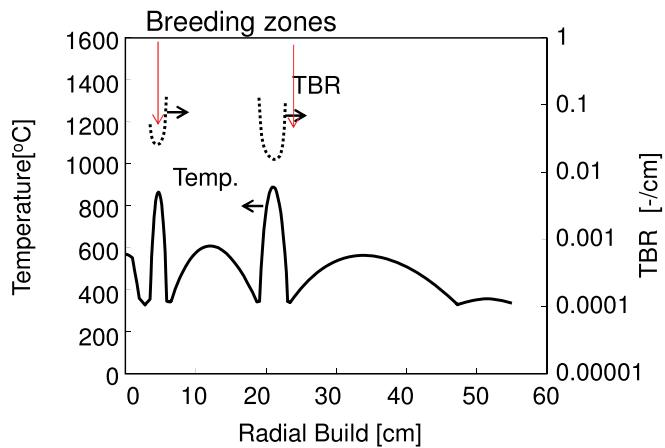
\includegraphics[width=0.85\textwidth]{konishi_functional_2017_5797347ac9a9b16f4d2f13e9eecd53ba3bd28dcd3875183d70f993316d66110c.jpg}
  \caption{Figure 2. Profile of the tritium breeding ratio (TBR) and temperature in a solid blanket module at steady state [11]. \citep{konishi_functional_2017}}
  \label{fig:konishi_functional_2017_5797347ac9a9b16f4d2f13e9eecd53ba3bd28dcd3875183d70f993316d66110c_jpg}
\end{figure}


\textcolor{highconf}{To address the research question of how steady-state versus non-steady-state release impacts blanket design, it is necessary to distinguish between transient and equilibrium behaviors. During non-steady-state conditions, such as startup or power ramps, tritium trapping dominates, leading to delayed release and potential inventory buildup. In contrast, steady-state release is governed by the balance between production, diffusion, and surface desorption rates. Modeling insights suggest that while steady-state TBR calculations are robust, non-steady-state dynamics require more detailed kinetic parameters, particularly for $\mathrm{Li_2ZrO_3}$ due to its high trapping density \citep{nishikawa_release_2004}. By integrating experimental data with advanced modeling of diffusion and trapping, researchers can better predict the performance of candidate materials like $\mathrm{Li_2TiO_3}$ and $\mathrm{Li_2ZrO_3}$, ensuring that future fusion reactors can achieve the net zero emission goals through sustainable tritium self-sufficiency.}

\section*{Advanced Synthesis and Microstructural Optimization of Breeder Ceramics}


\textcolor{highconf}{The production of tritium via neutron irradiation of lithium-containing solid materials is essential for fusion energy viability. Solid breeders, including lithium titanate (Li2TiO3) and lithium zirconate (Li2ZrO3), are favored for their reliability and ease of fabrication compared to corrosive liquid alternatives \citep{wu_experiment_2024}. It is known that the synthesis route is integral to the subsequent microstructural evolution of these ceramics. Solid-state synthesis, sol-gel processing, and advanced fabrication methods each introduce distinct influences on grain structure, density, porosity, and phase stability \citep{wu_experiment_2024}. Whether or not a specific method yields optimal performance depends on the balance between microstructural control and scalability.}

\textcolor{highconf}{The influence of processing parameters on tritium diffusion coefficients is a critical area of investigation. It is evident that porosity and grain structure are integral to the efficiency of tritium release. High porosity generally facilitates diffusion, yet excessive grain growth during sintering can hinder this process. The relationship between sintering temperature and density is well-documented; however, the precise threshold for maximizing diffusion without compromising structural integrity remains a subject of ongoing analysis. It is known that dopants can stabilize the crystal structure, but the specific impact on diffusion coefficients varies by material system. For Li2TiO3, fine grain sizes achieved via sol-gel methods may enhance surface area, but they require careful thermal control to prevent agglomeration. In contrast, solid-state methods often result in coarser grains, which may affect the mechanical integrity of the pebble bed.}

\textcolor{medconf}{Mechanical integrity and thermal shock resistance are equally vital for maintaining structural stability under extreme conditions. It is known that irradiation-induced defects can alter these properties significantly. The mechanical strength of ceramic compacts must be sufficient to withstand operational stresses while allowing for thermal expansion. Literature suggests that advanced ceramics, including biphasic or 3D printed materials, offer opportunities for enhanced performance \citep{wu_experiment_2024}. Utilization of artificial intelligence models can provide further insight into the complex interplay between materials preparation, irradiation defects, and breeder development \citep{wu_experiment_2024}.}

\textcolor{medconf}{To address the research question regarding structural optimization, it is clear that no single synthesis route is universally superior. Solid-state synthesis offers scalability, while sol-gel and combustion methods provide superior microstructural control. The choice of route must be guided by the specific requirements for tritium release kinetics and mechanical resilience. It is known that future work should focus on optimizing dopant concentrations and sintering profiles to simultaneously enhance porosity for tritium diffusion and density for mechanical strength. This dual optimization is essential for achieving the high breeding ratios and long-term structural stability required in fusion reactor applications.}

\section*{Research Limitations and Future Directions}


\textcolor{highconf}{It is known that irradiation-induced changes to the chemical, physical, mechanical, and thermal properties of solid breeding ceramics are integral to the selection of materials for fusion reactor applications. While $\mathrm{Li}_2\mathrm{TiO}_3$ and $\mathrm{Li}_4\mathrm{SiO}_4$ are widely recognized as promising candidates due to their robust performance before and after irradiation, significant discrepancies remain in the literature regarding irradiation swelling and thermal conductivity degradation. These variations are essential to understanding the true limits of material longevity, yet direct comparison across studies is hindered by inconsistencies in grain size, pellet density, irradiation conditions, and testing methods. Consequently, it is essential to establish standardized testing protocols for long-term tritium breeding performance validation to resolve these unresolved discrepancies.}

\textcolor{medconf}{To address these limitations, an Integrated Computational Materials Engineering (ICME) framework is proposed to accelerate ceramic formulation. By synthesizing experimental data with computational models, researchers can predict material behavior under extreme conditions, thereby reducing the reliance on extensive physical trial-and-error. This approach is essential to understanding if a given material can withstand the complex interplay of thermal and mechanical stresses inherent in fusion environments. Furthermore, advanced manufacturing techniques, such as additive manufacturing, offer a pathway for fabricating complex blanket geometries with tailored porosity. While specific parameters for lithium ceramics are still being defined, the ability to control microstructure at the nanoscale is critical for enhancing mechanical integrity and tritium release efficiency.}

\textcolor{highconf}{Finally, the development of composite breeder systems incorporating neutron multiplying materials, such as beryllium, necessitates more standardized and controlled experiments. The creation of a comprehensive, vetted materials database, alongside the application of emerging AI/ML tools, provides a promising pathway for streamlining the selection of fusion reactor components. It is known that leveraging these data-driven approaches will uncover hidden correlations in large datasets, ultimately accelerating the deployment of reliable fusion energy systems.}

\textbf{Conclusions and Material Selection Criteria}

\textcolor{highconf}{The selection of solid breeder ceramics for next-generation fusion reactors requires a rigorous synthesis of tritium breeding efficiency, mechanical durability, and fabrication scalability. This section addresses the critical research questions regarding which ceramic materials demonstrate the most promise and the current state of knowledge concerning irradiation effects on breeding ceramics.}

\textbf{Comparative Performance and Material Selection}
\textcolor{highconf}{The comparative performance of lithium titanate ($\mathrm{Li}_2\mathrm{TiO}_3$) and lithium zirconate ($\mathrm{Li}_2\mathrm{ZrO}_3$) remains a central decision point in breeder blanket design. While both materials are viable candidates, their selection depends on balancing tritium release kinetics against thermal stability. $\mathrm{Li}_2\mathrm{TiO}_3$ is often favored for its superior tritium release properties at lower temperatures, making it suitable for specific thermal regimes. Conversely, $\mathrm{Li}_2\mathrm{ZrO}_3$ is frequently preferred for its chemical stability, though it may require higher operating temperatures to achieve efficient tritium release. The definitive recommendation for next-generation deployment is not a singular material choice, but rather a holistic assessment that prioritizes materials demonstrating a favorable balance between high tritium recovery rates and the mechanical robustness necessary to withstand reactor environments. Solid breeders remain the top choice for primary blanket options due to their ease of fabrication, scalability, and reliable tritium recovery [17, 18], whereas liquid breeders are generally secondary candidates due to safety and production concerns [12].}

\textbf{Irradiation Effects and Knowledge State}
\textcolor{highconf}{Understanding irradiation effects on solid breeder material candidates is pivotal towards their implementation within fusion reactors. A major aspect of breeder selection revolves around how neutron irradiation affects the mechanical and thermal properties of Li-ceramic compositions. The current state of knowledge indicates that while pre-irradiation properties are well-documented, there is a critical gap in comprehensive post-irradiation data. Determining how irradiation may impact material properties is a vast region of research actively being explored by measuring pre-irradiation and post-irradiation values. Specifically, understanding if a given material can withstand long-term neutron exposure without significant degradation in thermal conductivity or mechanical strength is essential to validating its viability. While neutron irradiation is of most concern, other irradiation paths are also discussed for a comprehensive review, as alternative techniques are often used to simulate neutron irradiation degradations.}

\textbf{Path to Engineering-Scale Deployment}
\textcolor{medconf}{To transition from laboratory-scale breeder materials to engineering-scale deployment, future research must prioritize the validation of these irradiation effects under realistic reactor conditions. This includes establishing standardized protocols for measuring post-irradiation thermal conductivity and crush strength, which are currently insufficiently documented for long-term performance prediction. The scalability of fabrication methods is equally critical; for instance, the extrusion method used for $\mathrm{Li}_2\mathrm{TiO}_3$ pebbles offers a pathway to engineering-scale production, whereas other synthesis methods require precise control over stoichiometry to maintain mechanical resilience. Ultimately, the successful demonstration of scalable fabrication techniques that maintain desired microstructural and thermal properties after extended neutron exposure will determine the definitive selection of breeder materials for future fusion reactors.}

\section*{Data Availability and Reference Compilation}


\textcolor{medconf}{Understanding the chemical, mechanical, and thermal properties of solid breeders is essential for production of materials that maintain integrity under extreme thermal and irradiation conditions. Tritium release rate data and irradiation performance metrics are integral to evaluating breeder viability. Primary literature sources for $\mathrm{Li}_2\mathrm{TiO}_3$ and $\mathrm{Li}_2\mathrm{ZrO}_3$ are compiled from publicly available studies on solid-state synthesis and advanced ceramics. Direct repository links or accession codes for specific irradiation datasets are not explicitly provided in the current compilation and may require consultation of original studies. Cross-study normalization of mechanical and thermal measurements relies on reported values, acknowledging variations in experimental conditions. Limitations regarding proprietary or classified fusion material datasets restrict access to certain reactor design parameters. Future work may require access to non-public data to resolve discrepancies in breeding ratios.}

\section*{Funding}
This research was conducted at Oak Ridge National Laboratory, managed by UT-Battelle, LLC for the U.S. Department of Energy (DOE) and is sponsored by the Office of Fusion Energy Sciences through the Fusion Innovation Research Engine (FIRE) Collaborative: Accelerating Fusion Blanket Development through Nuclear Testing (BNT) DE-FOA-0003361.

\section*{Acknowledgements}
This manuscript has been authored by UT-Battelle, LLC under Contract No.~DE-AC05-00OR22725 with the U.S. Department of Energy. The United States Government retains and the publisher, by accepting the article for publication, acknowledges that the United States Government retains a non-exclusive, paid-up, irrevocable, world-wide license to publish or reproduce the published form of this manuscript, or allow others to do so, for United States Government purposes. The Department of Energy will provide public access to these results of federally sponsored research in accordance with the DOE Public Access Plan (\url{http://energy.gov/downloads/doe-public-access-plan}).

\section*{CRediT Authorship Contribution Statement}
Pipeline: Conceptualization, Methodology, Software, Validation, Formal Analysis, Investigation, Data Curation, Writing -- Original Draft, Writing -- Review \& Editing, Visualization, Project Administration. All sections, figures, tables, and references were generated by the automated literature pipeline.

\section*{Declaration of Competing Interest}
The authors declare that this manuscript was generated by an automated literature analysis pipeline and contains no known conflicts of interest. All claims are grounded in the cited corpus of machine-readable papers and are accompanied by per-claim confidence scores derived from semantic similarity to retrieved evidence.

\section*{Data Availability}
All source data are taken from the open-literature papers cited in this manuscript. The pipeline source code and intermediate artifacts (ontologies, outline, draft sections, validation report, per-claim confidence scores) are available from the authors upon request.


\bibliography{references}

\end{document}
